\documentclass{article}

\usepackage{fontspec}
\usepackage{fullpage}
\usepackage{multicol}
\usepackage{multirow}
\usepackage{tikz}

\begin{document}

\newfontfamily\swfill{SuttonSignWritingFill.ttf}
\newfontfamily\swline{SuttonSignWritingLine.ttf}
\newcommand{\bul}{\hfil$\bullet$&}
\renewenvironment{glossary}{\begin{multicols}{5}\begin{center}}{\end{center}\end{multicols}}
\setcounter{secnumdepth}{0}
\setlength{\columnseprule}{1pt}

\section{Supplement For Lesson 6}

\begin{center}
\it
Objectives inspired by, vocabulary transcribed from, and sentences and story by Bill Vicars.

Handshape photos by Adam Frost.

No endorsement implied nor given by either.
\end{center}

\subsection{Objectives}

\begin{tabular}{p{1cm}p{14cm}}
\bul I have completed the objectives for this lesson.\\
\bul I am able to read the numbers 100--999.\\
\bul I am able to show the meaning and form of the symbol groups in the body category in order.\\
\bul I know which base symbols are in Symbol Groups contact and finger.\\
\bul I am able to draw the flat palmshape in all forms.\\
\bul I am able to draw and demonstrate what fill five means.\\
\bul I am able to read, write, and sign the ASL handshapes in symbol group four.\\
\bul I am able to recognize the vocabulary for this lesson.\\
\bul I am able to read the practice sentences for this lesson.\\
\bul I am able to read the practice story for this lesson.\\
\end{tabular}

\subsection{The Numbers 100 Through 999}

In SignWriting you will also see this simply as a vertical list of the digits for zero through nine for page numbers and similar contexts.
In fact, you are more likely to see these written that way because adjusting several dozen page numbers to make the two digit numbers look good is a viable amount of work, but doing that for hundreds of pages is not.

Regardless of those uses, you should be using the correct signs in speaking and in writing for these lessons.

\begin{center}
\begin{tabular}{*{5}{c}}
\textbf{100}&\textbf{200}&\textbf{300}&\textbf{400}&\textbf{500}\\
B519x515S16d20502x495S10020481x485&
B510x535S10e20493x465S11020491x508&
B512x534S11e20488x467S12220490x507&
B513x538S14420490x463S14520488x507&
B514x533S14c20487x468S15020489x502\\
\textbf{600}&\textbf{700}&\textbf{800}&\textbf{900}\\
B509x528S16d20492x508S18720491x473&
B511x526S16d20489x506S1a520490x474&
B511x526S16d20490x506S1bb20490x474&
B511x527S16d20490x507S1ce20489x474\\
\end{tabular}
\end{center}

\subsection{The Body Category}

The official name for this category also happens to be ``Body'' and it has only two base symbols in it.

\begin{center}
\begin{tabular}{ccc@{\hskip 5mm}ccc}
\textbf{Symbol}&&&\textbf{Symbol}\\
\textbf{Group}&\textbf{Name}&\textbf{Example}&\textbf{Group}&\textbf{Name}&\textbf{Example}\\
\textbf{27}&Trunk&B521x502S36d00479x498&\textbf{28}&Limbs&B512x512S37600488x489\\
\end{tabular}
\end{center}

\subsection{The Symbol Groups Contact and Finger}

In prior lessons we have only talked the types of symbols that are in these groups, primarily because we are and will be covering each of them in detail throughout these supplements.
From this point on, we will instead be all of the base symbols \emph{in order} to see how these symbols are organized.
The order will be important in things like dictionaries (touch single, then multiple, then between, then grasp single) but honestly the goal from this point is more about generally knowing which symbols are where, what they mean, and a \emph{general feel} for which order they are in.

The eleventh Symbol Group we informally call contact, and it's official name also happens to be contact.
Symbol Group Contact has all the different ways that touch happens while moving.

\begin{center}
\begin{tabular}{rcrc}
\textbf{Base Symbol}&\textbf{Example}&\textbf{Base Symbol}&\textbf{Example}\\
Touch Single   &B505x506S20500495x495&Touch Multiple &B511x506S20600489x495\\
Touch Between  &B509x508S20700491x493&Grasp Single   &B505x505S20800495x495\\
Grasp Multiple &B511x505S20900489x495&Grasp Between  &B509x508S20a00491x493\\
Strike Single  &B507x507S20b00494x494&Strike Multiple&B514x507S20c00486x494\\
Strike Between &B511x508S20d00490x493&Brush Single   &B506x506S20e00494x494\\
Brush Multiple &B513x506S20f00487x494&Brush Between  &B510x508S21000490x493\\
Rub Single     &B507x507S21100494x493&Rub Multiple   &B514x507S21200486x493\\
Rub Between    &B511x508S21300490x492&Surface Symbols&B508x503S21400493x498\\
Surface Between&B508x505S21500492x496\\
\end{tabular}
\end{center}

Each of the ``Between'' versions also has a ``Multiple Between'' version as an additional fill.

The twelfth Symbol Group we informally call finger, though it's official name is ``Finger Movement''.
Symbol Group Finger Movement (Finger) has all ways the fingers can move.

The directional movement forms, you may notice, have either one or two tails.
The reasons for this will be explored in future lessons.

\begin{center}
\begin{tabular}{rcrc}
\textbf{Base Symbol}&\textbf{Example}&\textbf{Base Symbol}&\textbf{Example}\\
Squeeze Large Single                     &B504x504S21600496x496&Squeeze Small Single                     &B503x503S21700497x497\\
Squeeze Large Multiple                   &B509x504S21800491x496&Squeeze Small Multiple                   &B507x503S21900493x497\\
Squeeze Sequential                       &B506x513S21a00494x488&Flick Large Single                       &B504x504S21b00496x496\\
Flick Small Single                       &B503x503S21c00497x497&Flick Large Multiple                     &B509x504S21d00491x496\\
Flick Small Multiple                     &B507x503S21e00493x497&Flick Sequential                         &B506x513S21f00494x488\\
Squeeze Flick Alternating                &B517x506S22000483x495&Hinge Movement, Up Down Large            &B506x504S22100494x497\\
Hinge Movement, Up Down Small            &B505x503S22200495x498&Hinge Movement, Up Sequential            &B510x518S22300490x483\\
Hinge Movement, Down Sequential          &B510x518S22400490x483&Hinge Movement, Up Down Alternating Large&B506x507S22500494x494\\
Hinge Movement, Up Down Alternating Small&B505x505S22600495x496&Hinge Movement, Side to Side Scissors    &B508x505S22700492x496\\
Finger Contact Movement, Wall Plane      &B505x505S22800495x495&Finger Contact Movement, Floor Plane     &B505x505S22900495x495\\
\end{tabular}
\end{center}

Before you can consider this lesson complete, you need to be able to list off the symbol groups as:
``one, two, three, four, five, six, seven, eight, nine, thumb;''
``contact, finger.''

One thing I want to point out that may have been missed is that there is now a semicolon (instead of a comma) after thumb.
The thirty base symbols are most often thought of as being in three groups of ten, and you should take full advantage of that as you learn the names of the base symbols in order.
The requirement is that you can list off the symbol groups, \emph{not} that you can list off the symbol groups \emph{in less that $x$ seconds}!

The first ten are handshapes --- which should have proven fairly easy for you.
The second ten are movements --- which will required a bit more work but we have some additional helps in the next lesson.
The third ten are categories three through seven --- you still remember those right?

More helps to come.

\subsection{The Flat Palmshape}

\begin{center}
\begin{tabular}{r*{6}{c}}
&\textbf{Fill 1}&\textbf{Fill 2}&\textbf{Fill 3}&\textbf{Fill 4}&\textbf{Fill 5}\textbf{Fill 6}\\
\multirow{2}{*}{\textbf{Right}}&
B506x514S15a00494x487&
B506x514S15a10494x487&
B506x514S15a20494x487&
B506x514S15a30494x487&
B506x514S15a40494x487&
B506x514S15a50494x487\\
&
\tikz{\draw[thick](5pt,15pt)--(10pt,10pt)--(10pt,0)--(0,0)--(0,10pt)--cycle;}&
\tikz{\draw[thick](5pt,15pt)--(10pt,10pt)--(10pt,0)--(0,0)--(0,10pt)--cycle;\draw[thick](5pt,15pt)--(5pt,0);\draw[thick](5pt,15pt)--(10pt,0);\draw[thick](10pt,10pt)--(5pt,0);}&
\tikz{\draw[thick](5pt,15pt)--(10pt,10pt)--(10pt,0)--(0,0)--(0,10pt)--cycle;\draw[thick](0,10pt)--(10pt,0);\draw[thick](10pt,10pt)--(0,0);}&
\tikz{\draw[thick](5pt,15pt)--(10pt,10pt)--(10pt,0)--(0,0)--(0,10pt)--cycle;\draw[thick](-5pt,7pt)--(15pt,7pt);}&
\tikz{\draw[thick](5pt,15pt)--(10pt,10pt)--(10pt,0)--(0,0)--(0,10pt)--cycle;\draw[thick](5pt,15pt)--(5pt,0);\draw[thick](5pt,15pt)--(10pt,0);\draw[thick](10pt,10pt)--(5pt,0);\draw[thick](-5pt,7pt)--(15pt,7pt);}&
\tikz{\draw[thick](5pt,15pt)--(10pt,10pt)--(10pt,0)--(0,0)--(0,10pt)--cycle;\draw[thick](0,10pt)--(10pt,0);\draw[thick](10pt,10pt)--(0,0);\draw[thick](-5pt,7pt)--(15pt,7pt);}\\
\textbf{Left}&
B506x514S15a08494x487&
B506x514S15a18494x487&
B506x514S15a28494x487&
B506x514S15a38494x487&
B506x514S15a48494x487&
B506x514S15a58494x487\\
\end{tabular}
\end{center}

\subsection{The Fifth Fill}

\subsubsection{Hand Symbols}

\begin{center}
B508x515S10040493x485 B508x515S10e40493x485 B512x515S11e40489x485
\end{center}

Any handshape symbol drawn in the fifth fill means that the signer's thumb is facing up.
For all the hand symbols, the empty portion represents the signer's palm and the filled portion represents the back of the hand.
So for fill five you would see your thumb --- leaving fill five half filled in.

\subsubsection{Everything Else}

\begin{center}
B518x518S30a40482x483
\end{center}

The fills for other categories tend to be a bit more variable.
Here we have the right eyebrow raised by itself.

\subsection{ASL Handshapes From Symbol Group Four}

The four handshapes in Symbol Group Four used by ASL in order are:
{\it
Four Fingers Spread;
Four Fingers Spread Bent;
Four Fingers Unit;
and Four Fingers Unit Bent;
}

\subsubsection{The Four Fingers Spread Handshape}

\begin{center}
\begin{tabular}{r*{6}{c}}
&\textbf{Fill 1}&\textbf{Fill 2}&\textbf{Fill 3}&\textbf{Fill 4}&\textbf{Fill 5}&\textbf{Fill 6}\\
\multirow{2}{*}{\textbf{Right}}&
B511x516S14400489x485&
B511x516S14410489x485&
B511x516S14420489x485&
B511x516S14430489x485&
B511x516S14440489x485&
B511x516S14450489x485\\
&
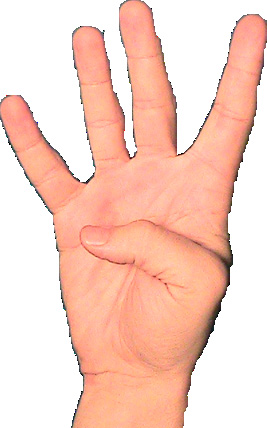
\includegraphics[scale=0.1]{images/04-01-1.jpg}&
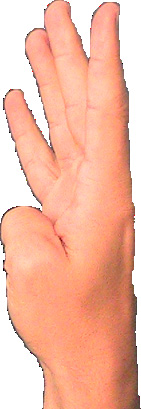
\includegraphics[scale=0.1]{images/04-01-2.jpg}&
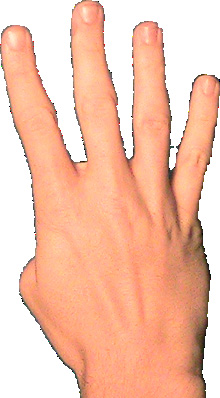
\includegraphics[scale=0.1]{images/04-01-3.jpg}&
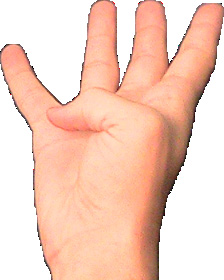
\includegraphics[scale=0.1]{images/04-01-4.jpg}&
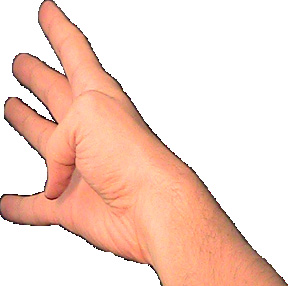
\includegraphics[scale=0.1]{images/04-01-5.jpg}&
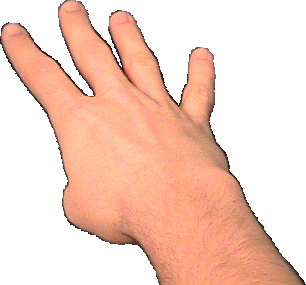
\includegraphics[scale=0.1]{images/04-01-6.jpg}\\
\textbf{Left}&
B511x516S14408489x485&
B511x516S14418489x485&
B511x516S14428489x485&
B511x516S14438489x485&
B511x516S14448489x485&
B511x516S14458489x485\\
\end{tabular}
\end{center}

\subsubsection{The Four Fingers Spread Bent Handshape}

\begin{center}
\begin{tabular}{r*{6}{c}}
&\textbf{Fill 1}&\textbf{Fill 2}&\textbf{Fill 3}&\textbf{Fill 4}&\textbf{Fill 5}&\textbf{Fill 6}\\
\multirow{2}{*}{\textbf{Right}}&
B512x516S14500489x485&
B512x516S14510489x485&
B512x516S14520489x485&
B512x516S14530489x485&
B512x516S14540489x485&
B512x516S14550489x485\\
&
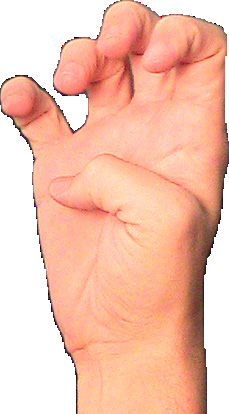
\includegraphics[scale=0.1]{images/04-02-1.jpg}&
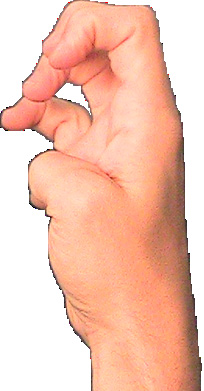
\includegraphics[scale=0.1]{images/04-02-2.jpg}&
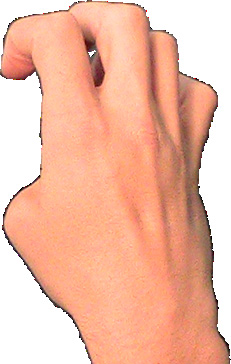
\includegraphics[scale=0.1]{images/04-02-3.jpg}&
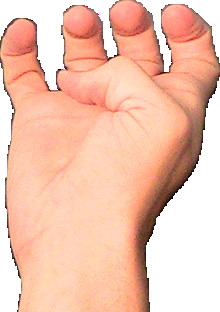
\includegraphics[scale=0.1]{images/04-02-4.jpg}&
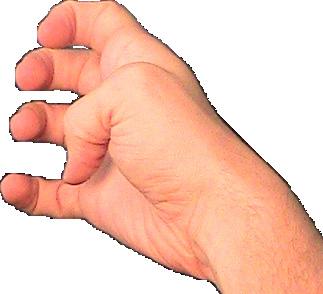
\includegraphics[scale=0.1]{images/04-02-5.jpg}&
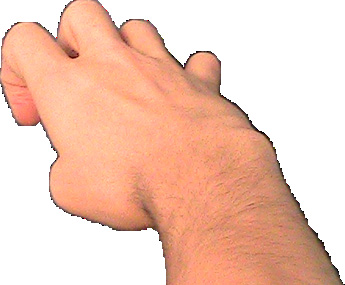
\includegraphics[scale=0.1]{images/04-02-6.jpg}\\
\textbf{Left}&
B512x516S14508489x485&
B512x516S14518489x485&
B512x516S14528489x485&
B512x516S14538489x485&
B512x516S14548489x485&
B512x516S14558489x485\\
\end{tabular}
\end{center}

\subsubsection{The Four Fingers Unit Handshape}

\begin{center}
\begin{tabular}{r*{6}{c}}
&\textbf{Fill 1}&\textbf{Fill 2}&\textbf{Fill 3}&\textbf{Fill 4}&\textbf{Fill 5}&\textbf{Fill 6}\\
\multirow{2}{*}{\textbf{Right}}&
B507x511S14700493x489&
B507x511S14710493x489&
B507x511S14720493x489&
B507x511S14730493x489&
B507x511S14740493x489&
B507x511S14750493x489\\
&
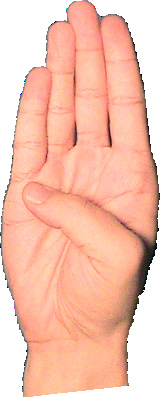
\includegraphics[scale=0.1]{images/04-03-1.jpg}&
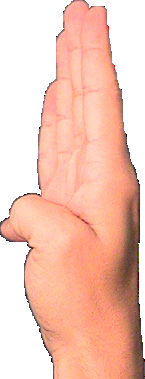
\includegraphics[scale=0.1]{images/04-03-2.jpg}&
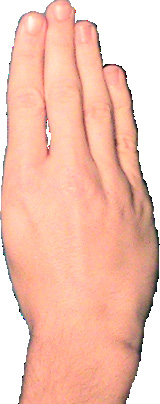
\includegraphics[scale=0.1]{images/04-03-3.jpg}&
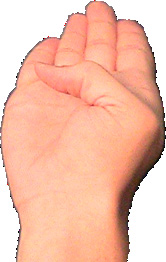
\includegraphics[scale=0.1]{images/04-03-4.jpg}&
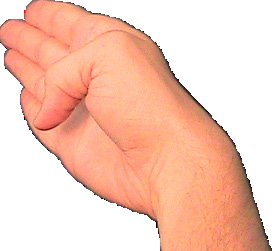
\includegraphics[scale=0.1]{images/04-03-5.jpg}&
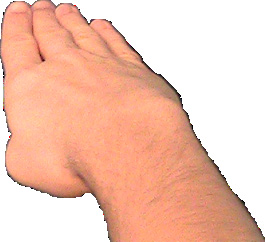
\includegraphics[scale=0.1]{images/04-03-6.jpg}\\
\textbf{Left}&
B507x511S14708493x489&
B507x511S14718493x489&
B507x511S14728493x489&
B507x511S14738493x489&
B507x511S14748493x489&
B507x511S14758493x489\\
\end{tabular}
\end{center}

\subsubsection{The Four Fingers Unit Bent Handshape}

\begin{center}
\begin{tabular}{r*{6}{c}}
&\textbf{Fill 1}&\textbf{Fill 2}&\textbf{Fill 3}&\textbf{Fill 4}&\textbf{Fill 5}&\textbf{Fill 6}\\
\multirow{2}{*}{\textbf{Right}}&
B508x508S14a00493x493&
B508x508S14a10493x493&
B508x508S14a20493x493&
B508x508S14a30493x493&
B508x508S14a40493x493&
B508x508S14a50493x493\\
&
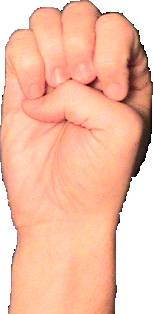
\includegraphics[scale=0.1]{images/04-04-1.jpg}&
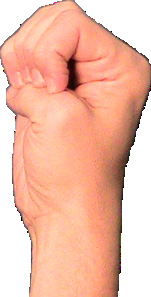
\includegraphics[scale=0.1]{images/04-04-2.jpg}&
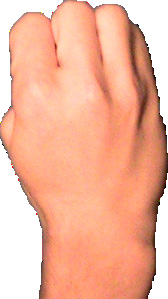
\includegraphics[scale=0.1]{images/04-04-3.jpg}&
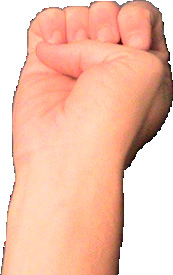
\includegraphics[scale=0.1]{images/04-04-4.jpg}&
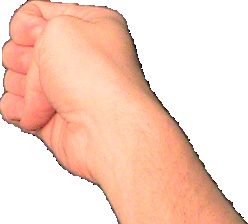
\includegraphics[scale=0.1]{images/04-04-5.jpg}&
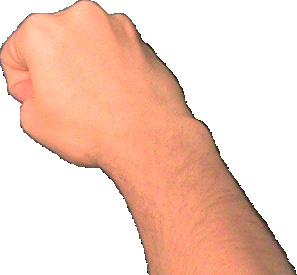
\includegraphics[scale=0.1]{images/04-04-6.jpg}\\
\textbf{Left}&
B508x508S14a08493x493&
B508x508S14a18493x493&
B508x508S14a28493x493&
B508x508S14a38493x493&
B508x508S14a48493x493&
B508x508S14a58493x493\\
\end{tabular}
\end{center}

\subsection{Vocabulary}

\begin{glossary}

\textbf{100}\\
AS10020S16d20M519x515S16d20502x495S10020481x485

\textbf{200}\\
AS10e20S11020M510x535S10e20493x465S11020491x508

\textbf{300}\\
AS11e20S12220M512x534S11e20488x467S12220490x507

\textbf{400}\\
AS14420S14520M513x538S14420490x463S14520488x507

\textbf{500}\\
AS14c20S15020M514x533S14c20487x468S15020489x502

\textbf{600}\\
AS18720S16d20M509x528S16d20492x508S18720491x473

\textbf{700}\\
AS1a520S16d20M511x526S16d20489x506S1a520490x474

\textbf{800}\\
AS1bb20S16d20M511x526S16d20490x506S1bb20490x474

\textbf{900}\\
AS1ce20S16d20M511x527S16d20490x507S1ce20489x474

\textbf{annual}\\
AS20340S20348S20500S20e00S26a00S10040M517x551S10040487x449S26a00483x484S20e00488x501S20340490x518S20348487x536S20500507x536

\textbf{before}\\
AS15d00S26604S36d00M547x530S36d00479x487S15d00528x470S26604527x500

\textbf{black}\\
AS10012S20e00S26506S2ff00M572x518S2ff00482x483S10012509x483S20e00542x484S26506557x482

\textbf{blue}\\
AS14710S2e008M511x528S14710491x473S2e008490x499

\textbf{brown}\\
AS14710S20e00S22a04S2ff00M533x549S2ff00482x483S14710519x496S22a04519x534S20e00519x520

\textbf{color}\\
AS14c00S22520S2ff00M518x565S14c00488x534S22520484x520S2ff00482x483

\textbf{current}\\
AS19a00S19a08S22a24M534x520S22a24494x505S19a00506x480S19a08467x480

\textbf{daily}\\
AS1f710S20e00S26a00S2ff00M540x518S2ff00482x483S1f710520x494S20e00519x478S26a00513x464

\textbf{dictionary}\\
AS10150S15a3aS20e00S26502M532x518S15a3a505x506S20e00490x495S10150510x483S26502468x496

\textbf{draw}\\
AS19210S15a06S22b05M521x524S15a06487x477S19210500x489S22b05479x500

\textbf{every day}\\
AS1f710S20e00S26a00S2ff00M540x518S2ff00482x483S1f710520x494S20e00519x478S26a00513x464

\textbf{far in the future}\\
AS15a10S2b800S34700M536x518S2b800511x454S15a10524x487S34700482x483

\textbf{finish}\\
AS14c00S14c08S2df08S2df10S2fb00M529x532S14c00506x501S14c08472x501S2df08507x476S2df10472x476S2fb00490x469

\textbf{future}\\
AS15a10S2ff00S2b700M534x518S2ff00482x483S15a10522x485S2b700513x453

\textbf{green}\\
AS1f000S2e230M516x526S1f000484x474S2e230497x494

\textbf{last year}\\
AS20340S20348S20500S10000S2b705S36d00M538x532S2b705524x508S36d00479x469S20340498x490S20348494x507S20500483x496S10000520x475

\textbf{later}\\
AS15a10S2ff00S2b700M534x518S2ff00482x483S15a10522x485S2b700513x453

\textbf{long}\\
AS10012S20e00S23800S37606M532x538S37606468x462S10012502x523S20e00492x508S23800476x481

\textbf{long ago}\\
AS14c00S22510S2b705S2f800S2f804S36e10M553x544S36e10480x491S14c00521x470S22510522x456S2b705528x511S2f800515x505S2f804515x533

\textbf{look up}\\
AS1f521S15a36S20e00S22a01M522x519S15a36494x507S1f521500x491S20e00489x492S22a01478x481

\textbf{next year}\\
AS20340S20348S20500S20e00S26500S10040M514x549S20340499x518S20348493x534S20500486x521S20e00495x502S10040494x451S26500494x483

\textbf{now}\\
AS19a00S19a08S22a24M534x520S22a24494x505S19a00506x480S19a08467x480

\textbf{old}\\
AS16d40S22a04S20340S20500S30004M521x577S30004482x483S16d40490x521S20500511x517S22a04495x544S20340494x562

\textbf{orange}\\
AS16d10S21600S33b00M518x553S21600497x545S16d10492x520S33b00482x483

\textbf{page}\\
AS1f521S15a36S20e00S22a01M522x519S15a36494x507S1f521500x491S20e00489x492S22a01478x481

\textbf{paper}\\
AS15d51S15d3aS20e00S26a01S20e00M528x530S15d3a497x496S15d51505x507S20e00492x481S26a01473x471S20e00483x491

\textbf{past}\\
AS15d00S26604S36d00M547x530S36d00479x487S15d00528x470S26604527x500

\textbf{present}\\
AS19a00S19a08S22a24M534x520S22a24494x505S19a00506x480S19a08467x480

\textbf{previously}\\
AS15d00S26604S36d00M547x530S36d00479x487S15d00528x470S26604527x500

\textbf{red}\\
AS10000S20e00S22a04S21600S33b00M526x552S21600515x544S33b00482x483S20e00514x514S22a04513x528S10000487x511

\textbf{self}\\
AS1f710S20600M511x515S20600489x504S1f710491x485

\textbf{someday}\\
AS15a10S2ff00S2b900M534x518S2ff00482x483S15a10522x485S2b900508x452

\textbf{today}\\
AS19a00S19a08S22a24M534x520S22a24494x505S19a00506x480S19a08467x480

\textbf{tomorrow}\\
AS1f710S20e00S26500S2ff00M540x518S2ff00482x483S1f710520x494S20e00519x478S26500517x460

\textbf{wait}\\
AS14c30S14c38S22520S22520S2fb00M535x529S14c30508x486S14c38471x498S22520503x471S22520466x484S2fb00484x475

\textbf{when}\\
AS10012S10019S2e708M536x522S10019464x492S10012487x492S2e708521x486S20500476x478

\textbf{white}\\
AS14c02S20500S26500S18501M517x535S14c02484x503S26500498x485S18501490x466S20500502x524

\textbf{will}\\
AS15a10S2b800S34700M536x518S2b800511x454S15a10524x487S34700482x483

\textbf{year}\\
AS20340S20348S2e734S20500M515x532S20340500x499S20348493x517S2e734495x468S20500486x504

\textbf{yellow}\\
AS19a10S2e230M514x530S19a10486x471S2e230490x498

\end{glossary}

\subsection{Practice Sheet 6.A}

\begin{multicols}{5}
\begin{center}

M508x515S10000493x485 % 1
M536x504S38800464x496 % .
M507x523S15a28494x496S26500493x477 % your
M540x543S1c507499x518S20600518x508S2ff00482x483 % favorite
M518x565S14c00488x534S22520484x520S2ff00482x483 % color
M537x504S38700463x496 % ,
M518x518S30c00482x483 % \?
M553x518S2fb04492x512S26c0a538x483S26c12448x488S14c39468x483S14c31506x483 % what
M536x507S38900464x493 % ?
\vfil
\columnbreak

M508x515S10e00493x485 % 2
M536x504S38800464x496 % .
M522x525S11541498x491S11549479x498S20600489x476 % name
M516x525S10000492x495S2e806484x475 % something
M521x517S1f710479x502S26a07500x483 % itself
M572x518S2ff00482x483S10012509x483S20e00542x484S26506557x482 % black
M517x535S14c02484x503S26500498x485S18501490x466S20500502x524 % white
M536x504S38800464x496 % .
\vfil
\columnbreak

M512x515S11e00489x485 % 3
M536x504S38800464x496 % .
M518x518S30a00482x483 % y/n
M510x523S10040495x493S26500491x478 % you
M516x540S1bb02488x461S14c02484x517S20e00499x502S26500499x483 % like
M518x565S14c00488x534S22520484x520S2ff00482x483 % color
M533x549S2ff00482x483S14710519x496S22a04519x534S20e00519x520 % brown
M536x507S38900464x493 % ?
\vfil
\columnbreak

M511x516S14400489x485 % 4
M536x504S38800464x496 % .
M518x518S30a00482x483 % y/n
M510x523S10040495x493S26500491x478 % you
M521x524S15a06487x477S19210500x489S22b05479x500 % draw
M518x585S2ff00482x483S15a00494x509S22a04494x539S15a39479x557S15a3f494x562 % good
M536x507S38900464x493 % ?
\vfil
\columnbreak

M512x516S14c00489x485 % 5
M536x504S38800464x496 % .
M518x518S30a00482x483 % y/n
M507x523S15a28494x496S26500493x477 % your
M518x541S2ff00482x483S14c10466x457S14c10465x510S20500494x471S20500494x519S22a00466x492 % parents
M535x531S10140504x469S10148484x469S20500498x473S28905508x504S2891d466x504S2fb04494x525 % divorce
M536x507S38900464x493 % ?
\vfil

\end{center}
\end{multicols}

\subsection{Practice Sheet 6.B}

\begin{multicols}{5}
\begin{center}

M509x515S18720491x486 % 6
M536x504S38800464x496 % .
M518x518S30a00482x483 % y/n
M510x523S10040495x493S26500491x478 % you
M529x532S14c00506x501S14c08472x501S2df08507x476S2df10472x476S2fb00490x469 % finish
M518x564S26500492x549S1e301486x518S2ff00482x483 % observe
M542x523S10058459x493S14c10482x477S20500476x501S2a502509x490 % movie
M536x511S38a00464x490 % :
M536x511S38a00464x490 % :
M536x507S38900464x493 % ?
\vfil
\columnbreak

M511x514S1a520490x486 % 7
M536x504S38800464x496 % .
M518x518S30a00482x483 % y/n
M510x523S10040495x493S26500491x478 % you
M539x519S2ff00482x483S10011518x489S20500510x474 % think
M534x518S2ff00482x483S15a10522x485S2b700513x453 % future
M510x523S10040495x493S26500491x478 % you
M546x518S2ff00482x483S18510521x490S18518452x493S26500525x468S26510458x469 % teach
M510x508S1f720490x493 % a
M508x508S20320493x493 % s
M512x515S1dc20488x485 % l
M536x507S38900464x493 % ?
\vfil
\columnbreak

M511x514S1bb20490x486 % 8
M536x504S38800464x496 % .
M518x518S30a00482x483 % y/n
M507x523S15a28494x496S26500493x477 % your
M521x521S11559480x496S20900494x479S11850498x494 % chair
M516x526S1f000484x474S2e230497x494 % green
M536x507S38900464x493 % ?
\vfil
\columnbreak

M511x515S1ce20489x485 % 9
M536x504S38800464x496 % .
M518x518S30c00482x483 % \?
M521x577S30004482x483S16d40490x521S20500511x517S22a04495x544S20340494x562 % old
M510x523S10040495x493S26500491x478 % you
M536x507S38900464x493 % ?
\vfil
\columnbreak

M513x528S2a538494x472S1f540488x504 % 10
M536x504S38800464x496 % .
M518x518S30c00482x483 % \?
M523x535S2ea48483x510S10011502x466S2ea04508x500S10019477x475 % sign (as in ``signing'')
M509x515S18720491x486 % w
M510x508S1f720490x493 % a
M511x510S19220490x491 % i (letter)
M508x510S1fb20493x491 % t
M536x507S38900464x493 % ?
\vfil

\end{center}
\end{multicols}

\subsection{Practice Sheet 6.C}

\begin{multicols}{5}
\begin{center}

M512x520S10000489x490S21d00494x480 % 11
M536x504S38800464x496 % .
M510x523S10040495x493S26500491x478 % you
M520x522S1f502505x498S1f50a480x498S22a20493x478 % live
M518x518S30c00482x483 % \?
M562x520S20500458x480S15a19439x494S15a11463x494S26526496x498S15a19514x497S15a11539x496S20500533x480 % city
M536x507S38900464x493 % ?
\vfil
\columnbreak

M509x521S10e00491x491S21d00491x480 % 12
M536x504S38800464x496 % .
M510x523S10040495x493S26500491x478 % you
M520x522S1f502505x498S1f50a480x498S22a20493x478 % live
M515x519S10047485x498S26507501x481 % 3rd person
M518x518S30c00482x483 % \?
M532x538S37606468x462S10012502x523S20e00492x508S23800476x481 % long
M536x507S38900464x493 % ?
\vfil
\columnbreak

M513x519S22114487x481S12d00489x489 % 13
M536x504S38800464x496 % .
M518x518S30a00482x483 % y/n
M510x523S10040495x493S26500491x478 % you
M534x543S14c30507x457S14c38469x458S15030508x512S15038467x511S26524493x493 % want
M525x526S10018476x477S10018497x496S2882a503x475 % go
M530x546S2ff00482x483S18517503x519S20500493x519S22a07515x511S20500520x494 % home
M535x522S22f14466x501S22f04510x501S2fb04494x516S18215468x479S1821d508x479 % now
M536x507S38900464x493 % ?
\vfil
\columnbreak

M513x515S14700493x493S22114487x486 % 14
M536x504S38800464x496 % .
M507x523S15a28494x496S26500493x477 % your
M528x530S15d3a497x496S15d51505x507S20e00492x481S26a01473x471S20e00483x491 % paper
M537x504S38700463x496 % ,
M518x518S30c00482x483 % \?
M553x518S2fb04492x512S26c0a538x483S26c12448x488S14c39468x483S14c31506x483 % what
M518x565S14c00488x534S22520484x520S2ff00482x483 % color
M536x507S38900464x493 % ?
\vfil
\columnbreak

M513x518S22114487x483S15d00494x491 % 15
M536x504S38800464x496 % .
M510x523S10040495x493S26500491x478 % you
M520x522S1f502505x498S1f50a480x498S22a20493x478 % live
M539x527S1e110506x473S1e118470x473S26606509x511S26612462x511 % big
M562x520S20500458x480S15a19439x494S15a11463x494S26526496x498S15a19514x497S15a11539x496S20500533x480 % city
M547x530S36d00479x487S15d00528x470S26604527x500 % past
M518x518S30a00482x483 % y/n
M510x523S10040495x493S26500491x478 % you
M536x507S38900464x493 % ?
\vfil

\end{center}
\end{multicols}

\subsection{Practice Sheet 6.D}

\begin{multicols}{5}
\begin{center}

M520x522S18700502x492S2e00e480x479 % 16
M536x504S38800464x496 % .
M518x518S30a00482x483 % y/n
M510x523S10040495x493S26500491x478 % you
M516x540S1bb02488x461S14c02484x517S20e00499x502S26500499x483 % like
M526x552S21600515x544S33b00482x483S20e00514x514S22a04513x528S10000487x511 % red
M556x537S20301466x474S20301511x464S28800527x500S2880c510x500S2880c544x500S28814464x501S28818445x501S28818482x502S2fb04496x531 % car
M536x507S38900464x493 % ?
\vfil
\columnbreak

M522x522S1a500501x494S2e00e478x478 % 17
M536x504S38800464x496 % .
M518x518S30a00482x483 % y/n
M540x518S2ff00482x483S1f710520x494S20e00519x478S26500517x460 % tomorrow
M510x523S10040495x493S26500491x478 % you
M525x526S10018476x477S10018497x496S2882a503x475 % go
M512x519S15a39489x496S15a5f488x496S20600489x482 % school
M536x507S38900464x493 % ?
\vfil
\columnbreak

M523x522S1bb00502x492S2e00e478x479 % 18
M536x504S38800464x496 % .
M510x523S10040495x493S26500491x478 % you
M525x526S10018476x477S10018497x496S2882a503x475 % go
M527x518S15a39497x482S18020497x503S20600473x498 % doctor
M537x504S38700463x496 % ,
M532x595S14c30505x542S14c38468x554S22520500x527S22520463x540S2fb00481x531S2e520490x568S35d00482x483 % wait long
M537x504S38700463x496 % ,
M510x523S10040495x493S26500491x478 % you
M521x548S11559480x453S11850498x456S22b24492x477S2a508492x515 % sit anxious
M518x518S30a00482x483 % y/n
M510x523S10040495x493S26500491x478 % you
M536x507S38900464x493 % ?
\vfil
\columnbreak

M524x522S1ce00502x490S2e00e477x479 % 19
M536x504S38800464x496 % .
M518x518S30c00482x483 % \?
M510x523S10040495x493S26500491x478 % you
M546x520S18557527x480S1855f492x480S28922454x505 % move here
M536x522S10019464x492S10012487x492S2e708521x486S20500476x478 % when
M536x507S38900464x493 % ?
\vfil
\columnbreak

M517x513S22114484x488S1f420488x498 % 20
M536x504S38800464x496 % .
M510x523S10040495x493S26500491x478 % you
M520x522S1f502505x498S1f50a480x498S22a20493x478 % live
M532x535S15a30475x466S15a30512x466S2fb04494x529S2e510468x498S2e508509x498 % here
M518x518S30c00482x483 % \?
M526x535S22a20494x501S14c08474x465S14c00503x465S20338478x520S20330508x520 % how many
M515x532S20340500x499S20348493x517S2e734495x468S20500486x504 % year
M536x507S38900464x493 % ?
\vfil

\end{center}
\end{multicols}

\subsection{Story 6}

\begin{multicols}{5}
\begin{center}
M538x532S2b705524x508S36d00479x469S20340498x490S20348494x507S20500483x496S10000520x475 % last year
M513x514S15a01490x486S20500487x503 % my
M525x539S15a11502x476S15a19476x476S20500495x462S23904505x501S2391c477x501S2fb04494x533 % house
M588x527S15a40461x475S15a48431x473S22104576x478S22104415x478S18048413x510S18040456x512S15a40561x475S15a48531x473S22104576x478S22104515x478S18048513x510S18040556x512S2d500487x493 % room room
M517x535S14c02484x503S26500498x485S18501490x466S20500502x524 % white
M510x508S1f720490x493 % a
M512x515S1dc20488x485 % l
M512x515S1dc20488x485 % l
M536x504S38800464x496 % .

M535x522S22f14466x501S22f04510x501S2fb04494x516S18215468x479S1821d508x479 % now
M515x532S20340500x499S20348493x517S2e734495x468S20500486x504 % year
M531x536S20300475x464S20300513x464S14c30507x505S14c38470x505S22a24495x486 % many
M518x565S14c00488x534S22520484x520S2ff00482x483 % color
M536x504S38800464x496 % .

M513x514S15a01490x486S20500487x503 % my
M539x593S15a17509x507S2ff00482x483S20500520x492S15a40512x541S15a48482x539S22104527x544S22104466x544S18048464x576S18040507x578 % bedroom
M511x528S14710491x473S2e008490x499 % blue
M536x504S38800464x496 % .

M513x514S15a01490x486S20500487x503 % my
M539x571S2ff00482x483S1dc50515x494S1dc0a500x547S1dc02474x530S20500487x557S22a03509x524 % sister
M539x593S15a17509x507S2ff00482x483S20500520x492S15a40512x541S15a48482x539S22104527x544S22104466x544S18048464x576S18040507x578 % bedroom
M514x530S19a10486x471S2e230490x498 % yellow
M536x504S38800464x496 % .

M538x568S1dc51508x466S1dc4a490x544S1dc42464x526S20500475x553S22b03501x512S2ff00482x483 % brother
M534x543S14c30507x457S14c38469x458S15030508x512S15038467x511S26524493x493 % want
M539x593S15a17509x507S2ff00482x483S20500520x492S15a40512x541S15a48482x539S22104527x544S22104466x544S18048464x576S18040507x578 % bedroom
M572x518S2ff00482x483S10012509x483S20e00542x484S26506557x482 % black
M537x504S38700463x496 % ,
M518x518S2ff00482x483S20500495x469S14c10468x453 % father
M518x549S30c00482x483S13f10486x534S2f900505x524S22114474x523 % no sternly
M536x504S38800464x496 % .

L518x518S30a00482x483 % y/n
L518x553S21600497x545S16d10492x520S33b00482x483 % orange
M536x507S38900464x493 % ?

R518x549S30c00482x483S13f10486x534S2f900505x524S22114474x523 % no sternly
M536x504S38800464x496 % .

L518x518S30a00482x483 % y/n
L533x549S2ff00482x483S14710519x496S22a04519x534S20e00519x520 % brown
M536x507S38900464x493 % ?

R518x518S32100482x483S2f900494x470 % think about it for a moment
R520x548S14020481x499S17620494x471S2f800482x453S2fa00497x541 % ok reluctant
M536x504S38800464x496 % .

M518x541S2ff00482x483S14c10466x457S14c10465x510S20500494x471S20500494x519S22a00466x492 % parents
M515x519S10047485x498S26507501x481 % 3rd person
M539x593S15a17509x507S2ff00482x483S20500520x492S15a40512x541S15a48482x539S22104527x544S22104466x544S18048464x576S18040507x578 % bedroom
M517x535S14c02484x503S26500498x485S18501490x466S20500502x524 % white
M536x504S38800464x496 % .

M518x520S1fb20482x490S27106503x480 % bathroom
M514x530S19a10486x471S2e230490x498 % yellow
M536x504S38800464x496 % .

M524x534S1ce20502x504S1ce28477x504S2df06502x476S2df1e478x476S2fb00494x467 % family
M538x527S15a40511x475S15a48481x473S22104526x478S22104465x478S18048463x510S18040506x512 % room
M516x526S1f000484x474S2e230497x494 % green
M536x504S38800464x496 % .

M515x523S15a20497x477S2d60c486x510 % our
M556x537S20301466x474S20301511x464S28800527x500S2880c510x500S2880c544x500S28814464x501S28818445x501S28818482x502S2fb04496x531 % car
M526x552S21600515x544S33b00482x483S20e00514x514S22a04513x528S10000487x511 % red
M536x504S38800464x496 % .

\end{center}
\end{multicols}

\end{document}

